\section{Pattern: Constraint Check Insertion}
\label{section:constraint-check}
\subsection{Motivation}
As mentioned before, Redex supports a few different forms of constraint checking; however, for the initial PyRedex implementation only the "equality of terms" constraint check is supported. For example, in the pattern \texttt{(number\_1 number\_1)} both terms bound to \texttt{number\_1} must be the same, meaning the term \texttt{(1 1)} does match the pattern but \texttt{(1 2)} does not.

However, since the current design of the \texttt{Match} class, explained in Section \ref{section:Match}, does not allow assigning multiple terms to the same pattern-variable, certain pattern-variables have to be renamed. Given $n$ occurrences of a pattern-variable, $n-1$ occurrences are to be renamed. After completion of pattern matching these $n-1$ pattern-variables must be removed from all returned \texttt{Match} instances.

Finally, actual equality checks have to be inserted. There are two obvious strategies that could be employed:

\begin{itemize}
\item Compare required pattern-variables \textit{after} matching a term against a pattern. The disadvantage of this strategy is that the pattern has to be matched entirely despite the fact that failure may happen very early in the matching process, thus resulting in useless work.

\item Compare required pattern-variables at the \textit{earliest} time possible, as pattern-variables become available. This is the strategy that PyPltRedex uses.
\end{itemize}

\subsection{Pattern-Variable Renaming}
Pattern variable $pv$ is renamed in the following manner: $\mathit{pv + \# + freshint()}$, $\mathit{freshint()}$ if $\mathit{freshint() > 0}$ otherwise $pv$. $\mathit{freshint}$ operation was defined previously in Section \ref{section:id-rewrite}. For example, assuming $\mathit{freshint()=0}$, renaming \texttt{m} results in \texttt{m}. Successive application of the renaming operation results in \texttt{$m\#1$}.

\subsection{Algorithm}
Since the algorithm is based in renaming (or modification) of pattern-variables, let $v^{\prime}$ be a new pattern-variable after modifying $v$. The pairs $(pv, pv^{\prime})$ need to be maintained in order to decide where to insert equality checks. Let $M$ be a set containing such pairs. Furthermore, to remove renamed pattern-variables after matching, the set $R$ containing such pattern-variables has to be maintained.

Given some pattern $p$, \Visit{$p$}. The following kinds of $p$ are of interest.
\begin{itemize}
\item $p=$\space \BuiltInPattern. Let $pv^{\prime}$ be a renamed variable and let $M=\{(pv, pv^{\prime})\}$. If $pv \neq pv^{\prime}$, $R=R \cup \{pv^{\prime}\}$. Return \BuiltInPattern[$tag$][$pv^{\prime}$][false] and $M$.
\item $p=$\space \NonTerminal. Let $pv^{\prime}$ be a renamed variable and let $M=\{(pv, pv^{\prime})\}$. If $pv \neq pv^{\prime}$, $R=R \cup \{pv^{\prime}\}$. Return \NonTerminal[$nt$][$pv^{\prime}$][false] and $M$.
\item $p=$\space \LiteralPattern \space contains no pattern-variables and thus $p$ and $\emptyset$ are returned.
\item $p=$\space \PatternRepeat. Let $p_r^{\prime}, M =$\Visit{$p_r$}. Return \PatternRepeat[$p_r^{\prime}$], $M$.
\item
$p=$\space \PatternSequence. If the sequence contains no child patterns, return $p$, $\emptyset$. Define \texttt{merge} operation that, given two sets $M_i, M_j$ returns two sets $M_k$ and $M_r$; this operation will be discussed below.
Let $p^{\prime}$ be the pattern sequence that replaces $p$.
Let $p_1^{\prime}, M_1$=\Visit{$p_1$}. Insert $p_1^{\prime}$ into $p^{\prime}$. For $p_i \in p_2, ..., p_n$, let $p_i^{\prime}, M_i$=\Visit{$p_i$}.
	\begin{enumerate}
	\item
	Insert $p_i^{\prime}$ into $p^{\prime}$.
	\item
	Let $M_1$, $M_r$ = \texttt{merge}($M_1$, $M_i$). For each pair of pattern-variables $(pv_a, pv_b) \in M_r$, insert \PatternCheckConstraint[$pv_a$][$pv_b$][false] into $p^{\prime}$.
	\end{enumerate}
Finally, return $p^{\prime}, M_1$.

\item
$p=$\space \PatternInHole.\\ Let $p_1^{\prime}, M_1$= \Visit{$p_1$} and $p_2^{\prime}, M_2$= \Visit{$p_2$}. Let $M, M_r$=\texttt{merge}($M_1$, $M_2$). For each pair of pattern-variables $(pv_a, pv_b) \in M_r$, let $c_i$=\PatternCheckConstraint[$pv_a$][$pv_b$][false]. Return \PatternInHole[$p_1^{\prime}$][$p_2^{\prime}$][$c_1$][$c_n$][false], $M$.
\end{itemize}

Finally, make an annotation \MakeAnnotation{$p$}{"PatConstraintCheckRemoveVars"}{$R$}.

\subsection{\texttt{merge} Operation}
Before proceeding with pattern traversal, \texttt{merge} operation needs to be defined. Given two sets $M_1$ and $M_2$ it produces two sets $M$ and $M_r$. Those sets are constructed in the following manner:

\begin{enumerate}
\item Let $M=\emptyset$ and $M_r=\emptyset$.
\item For each $(pv, pv^{\prime}) \in M_1$, find a pair $(pv, pv^{\prime\prime}) \in M_2$.
\begin{enumerate}
\item If such pair exists, then $M_r=M_r \cup \{(pv^{\prime},  pv^{\prime\prime})\}$ and $M=M \cup \{(pv,  pv^{\prime\prime})\}$.
\item Otherwise, $M=M \cup \{(pv,  pv^{\prime})\}$
\item For any other $(pv, pv^{\prime\prime}) \in M_2$ s.t.  $(pv, pv^{\prime}) \notin M_1$, $M=M \cup \{(pv,  pv^{\prime\prime})\}$
\end{enumerate}
\end{enumerate}

\subsection{Example}

\begin{figure}[ht]
	\centering
	\makebox[\textwidth][c] { 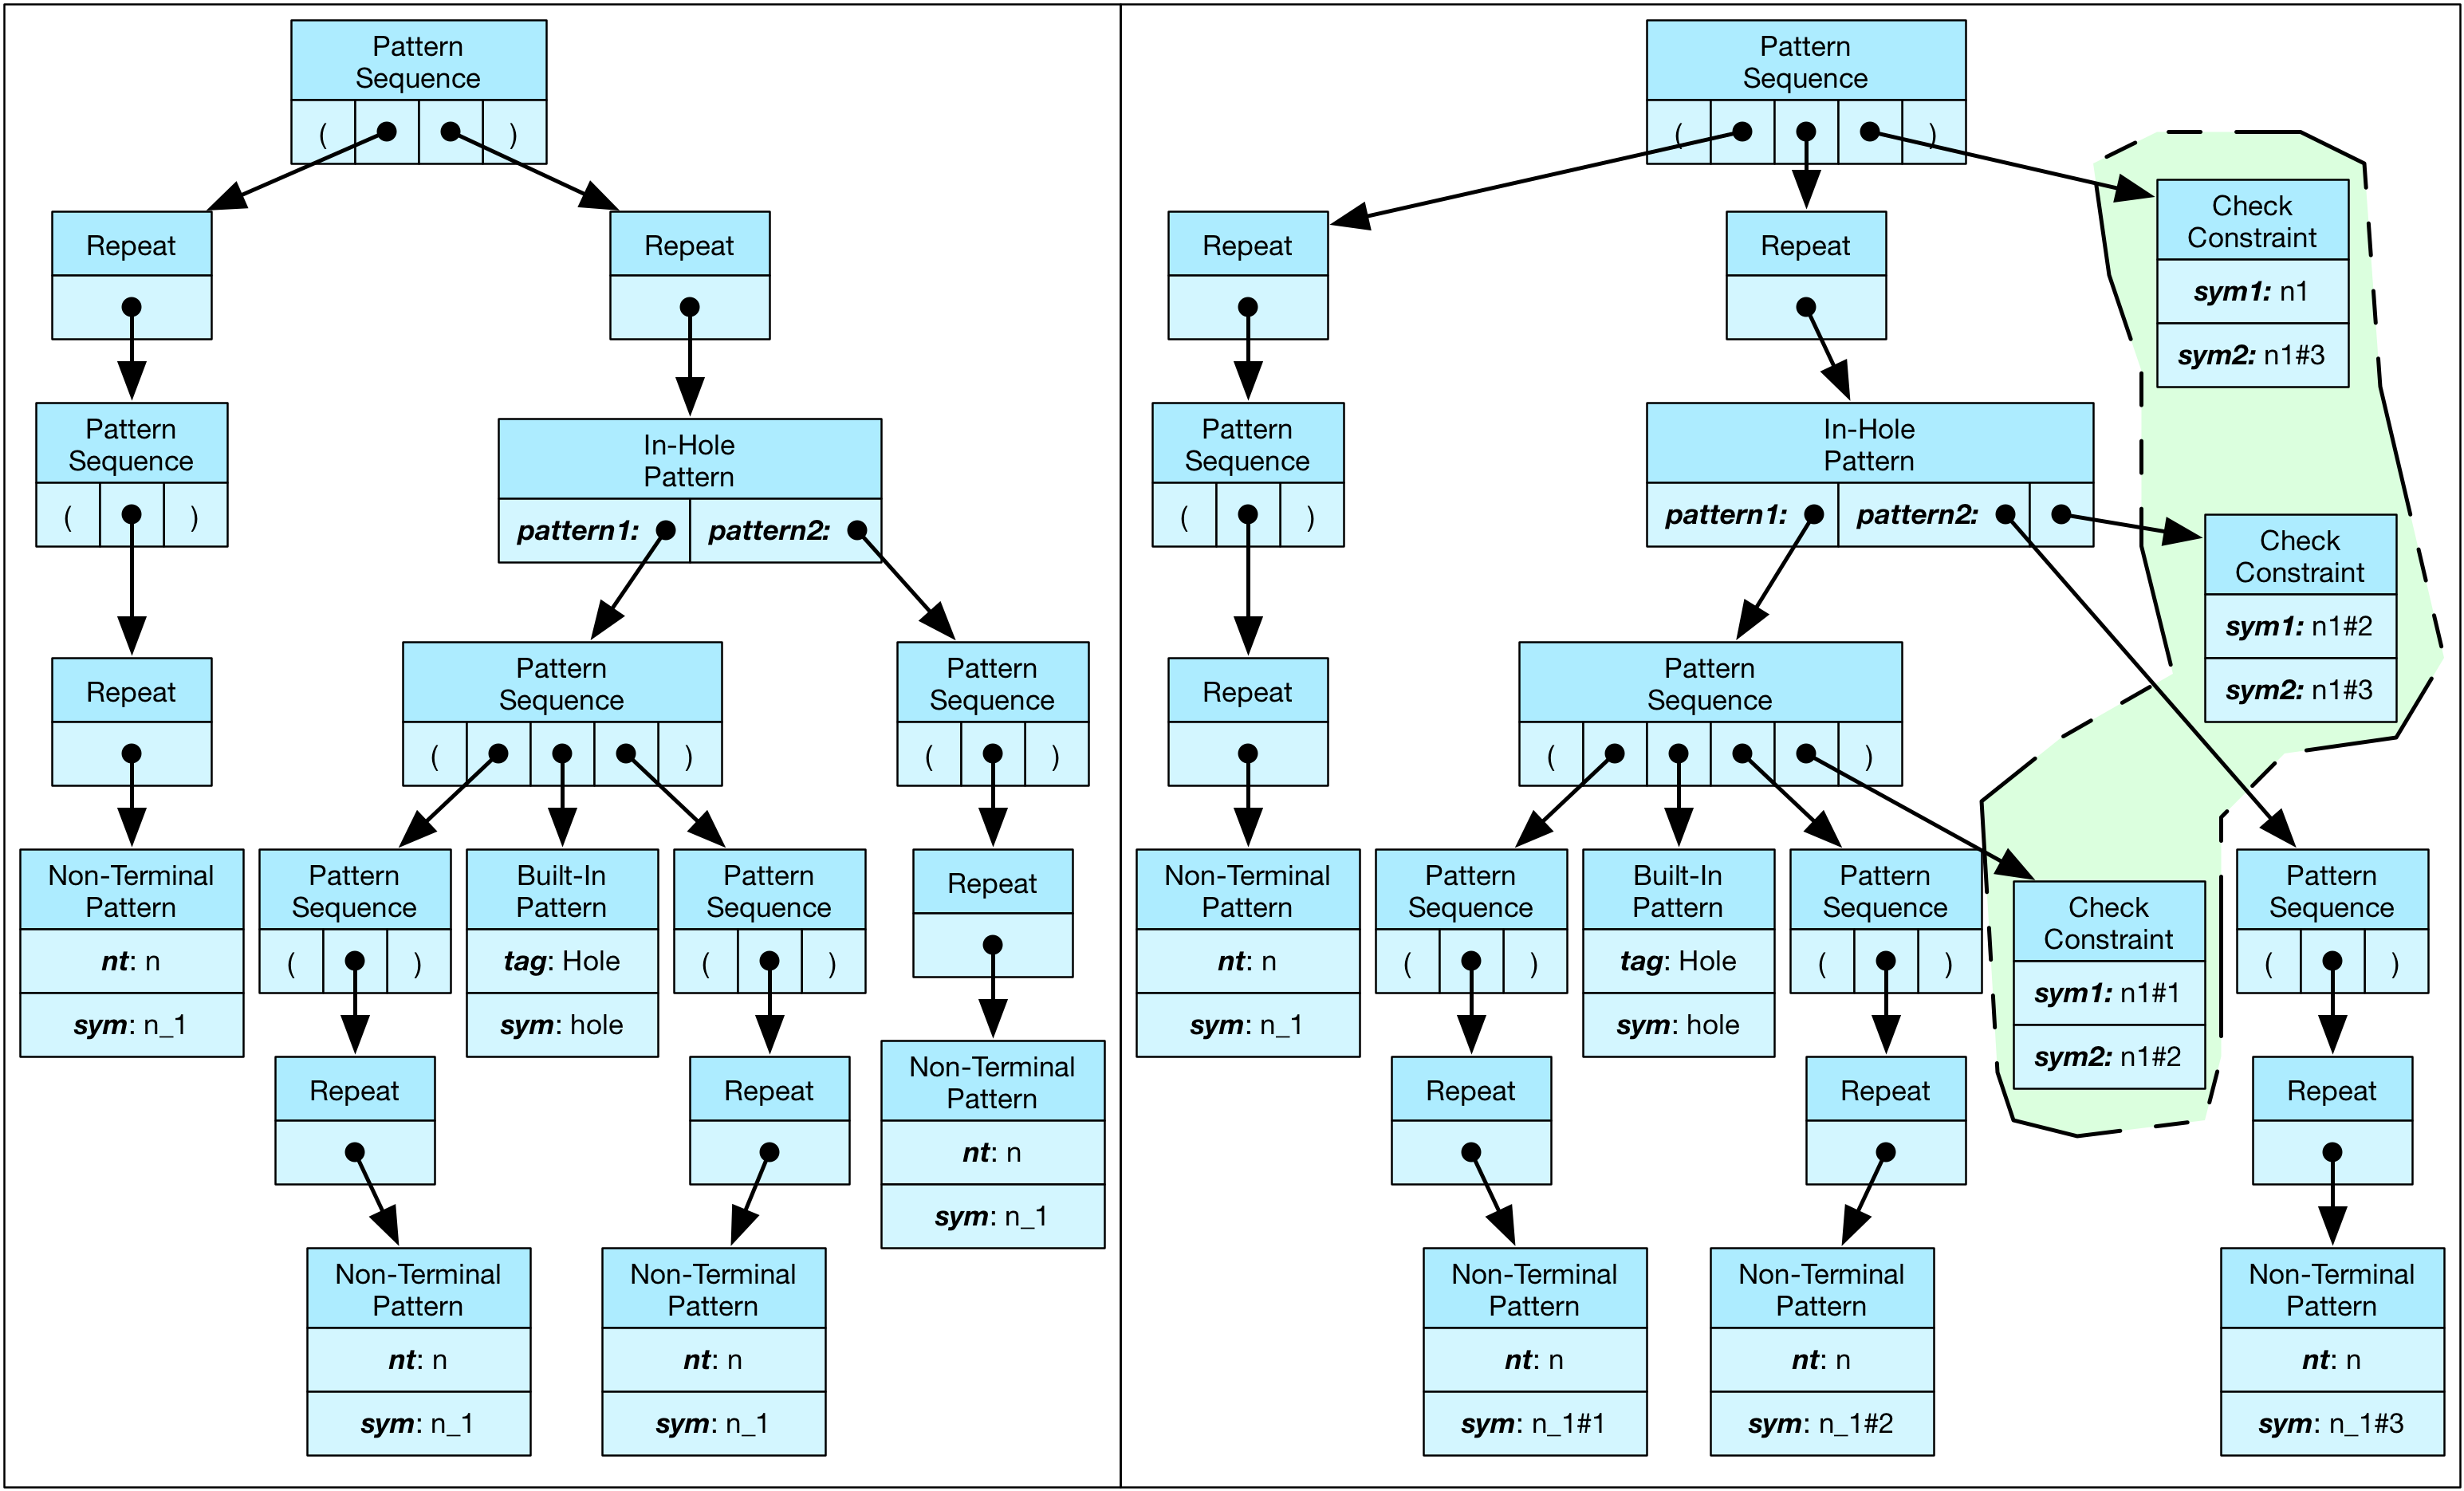
\includegraphics[scale=0.15]{transformation-pattern-constraintcheck.png} }
\caption{Applying transformation to pattern \texttt{((n\_1\ ...)\ ...\ (in-hole\ ((n\_1\ ...)\ hole\ (n\_1\ ...))\ (n\_1\ ...))\ ...)}, before and after.}
\label{transformation-pattern-constraintcheck}
\end{figure}

Figure \ref{transformation-pattern-constraintcheck} shows an effect of described transformation on the pattern \texttt{((n\_1\ ...)\ ...\ (in-hole\ ((n\_1\ ...)\ hole\ (n\_1\ ...))\ (n\_1\ ...))\ ...)}. Notice that all occurrences of \texttt{n\_1} have an ellipsis depth of two. The first occurrence of \texttt{n\_1} goes unmodified. Then, when processing the first pattern inside the \texttt{in-hole} pattern, there are two occurrences of \texttt{n\_1}. The first occurrence is renamed to \texttt{n\_1\#1}, the second to \texttt{n\_1\#2}, and \texttt{CheckConstraint(n\_1\#1, n\_1\#2)} is appended to the \texttt{PatternSequence}. The final occurrence of \texttt{n\_1} is seen in the second pattern of \texttt{in-hole} and is renamed to \texttt{n\_1\#3}. \texttt{CheckConstraint(n\_1\#2, n\_1\#3)} is then added to the \texttt{in-hole}. Finally after exiting \texttt{in-hole}, \texttt{CheckConstraint(n\_1, n\_1\#3)} is appended to \texttt{PatternSequence}.
